% -*- root: ./report.tex -*-

\chapter{Theory}
The topological quantum computer uses pairs of Majorana particles as its unit of computation (qubit).
In order to host Majorana modes in a system, one needs a material which has properties from a superconducting material, as well as from a semi-conducting material.
As this material does not seem to exist on its own, one creates a heterogeneous system.
I simple terms, this consists of a slab of superconductor and a strip of semiconductor.
By interfacing the two, one creates a region where all the necessary ingredients are present to realize Majorana's.

In this chapter, we first give a description of the normal (semi-conductor) and superconducting regions.
We then focus on what happens in a system where the two are interfaced.
Following that, we briefly explain what Majorana are, before introducing the implementation mainly relevant to this thesis.


\section{Normal region}
	Two important ingredients required for realizing Majorana fermions are strong spin-orbit coupling, and a strong interaction with the applied magnetic field.
	It is the normal conductor which brings these two physical effects to the mix.
	Note that the Hamiltonian of the normal region is the same for electrons and holes, except for the sign.
	The Hamiltonian terms provided in this section are relevant to the electron states.

    \subsection{Zeeman interaction}
    	The energy splitting of the two electron spin species due to magnetic field is called the Zeeman interaction.
    	It is modeled by:
    	\begin{equation}
    	H_\text{Z} = g \mu_B \vec{B} \cdot \vec{\sigma}
    	\end{equation}

    \subsection{Spin-orbit coupling}
	    An electron moving in an electric field will experience a small Zeeman field in its inertial frame as a relativistic effect~\cite{petersen_simple_2000}.
	    The resulting interaction, coupling the momentum and spin of electron, is known as spin orbit coupling.
	    Spin-orbit coupling can be approximated by adding a Rashba spin orbit coupling term in the Hamiltonian:
	    \begin{equation}
	    H_\text{Rashba} = \alpha (\ky \sigx - \kx \sigy) 
	    \end{equation}

\section{Superconducting region}
    The superconductor is responsible for ensuring particle-hole symmetry, as well as providing a `gapped' area in the bandstructure, isolating the zero-energy state.
    Superconductivity is a very complicated phenomenon, so we again provide only the background required for the understanding of this work.

    \subsection{Superconductivity}
		Superconductivity manifests itself as the complete lack of electrical resistance of a material.
		It is the result of the pairing of electrons close to the Fermi-energy, condensing into so-called Cooper pairs.
		The main parameter defining superconductivity is known as the superconducting order parameter, a complex number.
		The phase of this parameter is a macroscopic potential relative to ones choice of gauge.
		The magnitude of the superconducting order parameter, also referred to as the superconducting gap, quantifies the range around the Fermi-energy condensed into Cooper pairs.
		Because all electrons within a distance of the superconducting order parameter of the Fermi-energy are depleted in this way, charge transport only takes place via these quasiparticles.
		Scattering of these Cooper pairs is not allowed, resulting in perfect conduction.

		For the purpose of creating Majorana's, we are interested in two main aspects of superconductivity: the energy gap surrounding the Fermi energy (due to the depletion of states), and the electron-hole (/particle-hole) symmetry.
		We are thus not interested in the paired up electrons (Cooper pairs), and only wish to model the electronic (unpaired) modes.
		This can be achieved by modeling superconductivity with the Boguliubov de Gennes Hamiltonian:
		
		\begin{equation}
		\mathbf{H}_\text{BdG} = \begin{bmatrix} H & \Delta \\ \Delta^\dagger & H \end{bmatrix}
		\end{equation}

		The block matrix restricts the structure of the system in the electron-hole basis, and ensures particle-hole symmetry.
		For $\Delta \neq 0$ one indeed induces a identically sized gap in the spectrum.

	\subsection{Proximity effect}
		In order to create Majorana's, one needs a material with properties unique to both superconductors and semiconductors.
		However, if a superconductor is interfaced with a normal conductor, some of the properties belonging to the superconductor transfer to normal material.
		This effective transfer of properties to the normal material is known as the proximity effect.
		The characteristic distance governing the decay of the superconducting behavior is given by the superconducting coherence length, Eq.\eqref{eq:theory_sc_coherence_length}
		
		\begin{equation}
			\xi = \hbar \frac{v_\text{F}}{\Delta}
			\label{eq:theory_sc_coherence_length}
		\end{equation}


\section{Normal-superconducting junctions}
	As mentioned, the interesting physics occur when a normal conductor is interfaced with a superconductor.
	A single interface between a normal conductor and a superconductor is known as a NS junction.
	When one creates a sandwich, superconductor - normal - superconducting, we speak of a SNS junction.
	Even not considering topological phases, which are only present if the normal regions meets certain conditions, both have interesting physics which will be discussed first.


	\subsection{Andreev scattering}
		At the interface between a normal and superconducting region, electrons with energies below the superconducting gap undergo Andreev scattering.
		The quasiclassical microscopic explanation for this is as follows.
		An electron in the normal region with energy below the superconducting gap, incident on the normal-superconductor (NS) interface, is retro-reflected as a hole.
		This phenomenon is known as Andreev scattering, and occurs due to the coupling of electrons in a superconductor.
		Although a single electron initially enters the superconductor, it draws another electron (with opposite momentum) into the superconductor: forming a Cooper pair.
		The drawn in electron leaves behind a hole in the normal conductor, which essentially backtracks the motion of the initial electron, hence the term retro-reflection.
		The same effect, but opposite in particle type, holds for a hole entering the superconductor.

	\subsection{Andreev bound states}
		If the normal region is finite in the direction normal to the NS/SN interface, Andreev bound states form.
		This is true for both SNS and SN junctions.
		Quasiclassically, one can imagine electrons (and holes) in the normal region, with energies below the gap, bouncing back and forth the system.
		The corresponding eigenstates have energies below the gap, and are thus bound to the normal region.

	\subsection{Josephson junctions and supercurrent}
		An important device in the field of condensed matter physics is the Josephson junction.
		A Josephson junction consists of a normal region sandwiched in between two superconductors (SNS junction).
		The resulting Andreev bound states exhibit interesting physics, making the Josephson junction an important device.

		Although superconducting phase is relative to the choice of gauge, the difference of phase between two superconductors is in fact a physical quantity.
		A difference in superconducting phase in a Josephson junction, results in a flow of current between the two superconductors: a supercurrent.
		The relationship between superconducting phase and current is known as the current-phase relationship, and is in the most simple case a sinosoid.
		This relationship can be exploited to control the phase difference: it is a matter of inducing a current.

		An important measure in a Josephson junction is the Thouless energy.
		In the context of this work, the Thouless energy is inversely proportional to the travel time of an electron in a system, without interacting with the superconductor(s).
		As an example of its relevance, in a SNS junction with magnetic field, if the Zeeman field has an energy comparable to the Thouless energy, as the electron traverses the system from supercondcutor to superconductor, the spin will be flipped.
		
\section{Topology, Symmetry, and Majorana bound states}

	The Wikipedia definition of mathematical topology is as follows:
	
	\begin{quote}Topology can be formally defined as "the study of qualitative properties of certain objects (called topological spaces) that are invariant under a certain kind of transformation
	\cite{noauthor_topology_2018}
	\end{quote}

	Similarly, in condensed matter physics, topology refers to the study of properties of a system, which are guaranteed by particular symmetries of the Hamiltonian.
	These symmetries are present within a particular range of parameters, and any variation of those parameters within that range does not destroy these \emph{topologically protected} properties.
	
	Topology is relevant to the context of the system under study, because the emergence of seperated Majorana's is guaranteed within a continuous range of parameters.
	The presence of Majorana's is therefore topologically protected, as they will be unpurturbed by variations of parameters, within a certain range.
	For an infinite system, the system is said to be in the topological phase if Majorana's emerge once the system is cut to finite length.
	The system is considered to be in its trivial phase if the converse is true.
	The allocation of a system into one of its phases (in this case two) is quantitatively captured by its topological invariant.
	The relevant topological invariant is dependent on the symmetry class the system belongs to.
	In the case of the what is studied in this manuscript, the systems discussed belong to either symmetry class BDI or D.
	Any system which is in the BDI class is also contained within class D.
	The topological invariant of a class D system is binary: $-1$, corresponding to the topological phase, and $1$, corresponding to the trivial phase.
	The invariant of a BDI system can be any integer number, which also means there are more than two topological phases.
	More importantly, the transition of the system from one topological phase to the other means the system must undergo a gap closing.


	\subsection{Majorana bound states}
		We will give a very pragmatic description of Majorana bound states, insofar their relevance to this work.

		The Majorana state is a superposition of electrons and holes, and is its own anti-particle: exchanging electrons and holes yields the same state.
		The Majorana state carries no spin, charge, or energy, giving almost no degrees of freedom for it to interact with the environment.
		The Majorana state constitutes a single fermion, but is comprised of two Majorana's.
		In a finite, topological system, these two Majorana's are physically seperated, appearing at the edges.

		The lack of interaction, as well as the physical seperation of the state, makes it very robust against perturbations, but also difficult to detect.
		Luckily, the state's presence itself is measurable: the availability of a state contributes to the conduction at that energy.
		When measuring the conduction through a system with Majorana's present, one should thus encounter a rise in the conductance at zero energy: the zero bias peak.

	\subsection{Topological gap}
		The topological gap is defined as the energy gap between the Majorana state -- conveniently located at zero energy -- and the first available state.
		It's magnitude governs the protection of the system against perturbations causing the system to be lifted out of its ground state: the Majorana state.

	\subsection{Decay/Coherence length}
		The decay or coherence length of a Majorana pair is an important measure signifying the seperation of the two half-particles.
		A decay length larger or of equal size to the system dimensions will lead to overlap of the Majorana's, diminishing the desired robustness of the state.
		An overlap of the Majorana's will in fact lead to the system having a non-zero energy, its magnitude depending on the amount of overlap.
		A crude estimation of the size of an individual Majorana is:
		\begin{equation}
			\xi = \hbar \frac{v_\text{F}}{\Delta_\text{topological}}
			\label{eq:majorana_coherence_length}
		\end{equation}

		When the system is cut to a finite length, any overlap of the two Majorana's will lead to a non-zero energy.
		This decreases the robustness of the topological state and it is thus desirable that the Majorana decay length is significantly smaller than the system size.

\section{Two dimensional platform for Majoranas}

	\begin{figure}[!htb]
	\centering
	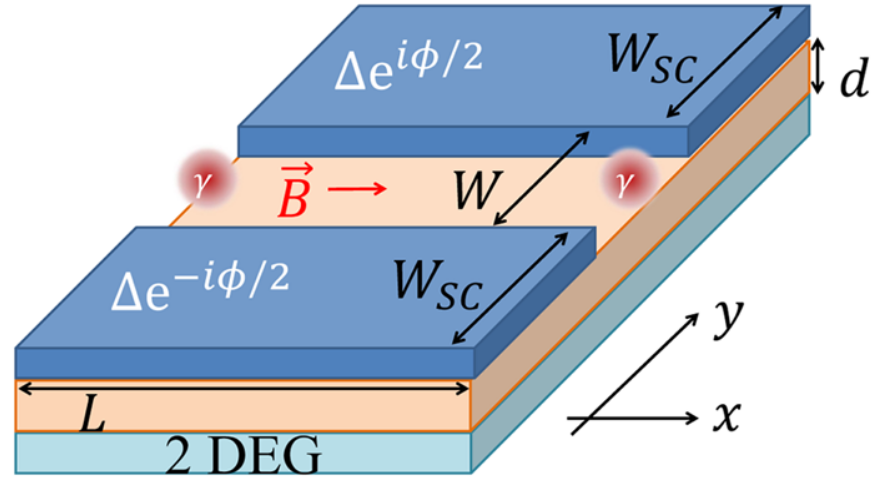
\includegraphics[width=0.5\columnwidth]{figures/pientka_system}
	\caption{System overview. Source\cite{pientka_topological_2017}}
	\label{fig:pientka_system}
	\end{figure}

	The earliest devices used to create a seperated pair of Majorana's were nanowires deposited onto a slab of superconducting material.
	A relatively new proposal is that of creating Majorana's in a planar Josephson junction~\cite{pientka_topological_2017}.
	An advantage of this system is that the phase difference between the superconductors can be used as a knob to switch the system from the topological state to the trivial state. 
	In addition, the presence of the second superconductor increases the topological gap of the system due to the proximity effect.

			

	\subsection{Phase diagram}
		As mentioned, the superconducting phase difference plays a critical role in the physics of the device.
		The topological phase diagram, as a function of magnetic field and superconducting phase, is depicted in Fig. \ref{fig:pientka_phase_diagram}.
		Without normal reflection (perfect Andreev reflection), the diagram has a diamond-like shape.
		The system is always topological when the superconducting phase is $pi$, or when the magnetic field is tuned to $(2N-1)$ times the Thouless energy(Eq. \ref{eq:theory:E_th})
		\begin{equation}
			E_\text{Th} = \frac{\hbar^2 \pi^2}{2 \meff \left( 2 W \right)^2}
			\label{eq:theory_E_th}
		\end{equation}
		
		\begin{figure}[!htb]
		\centering
		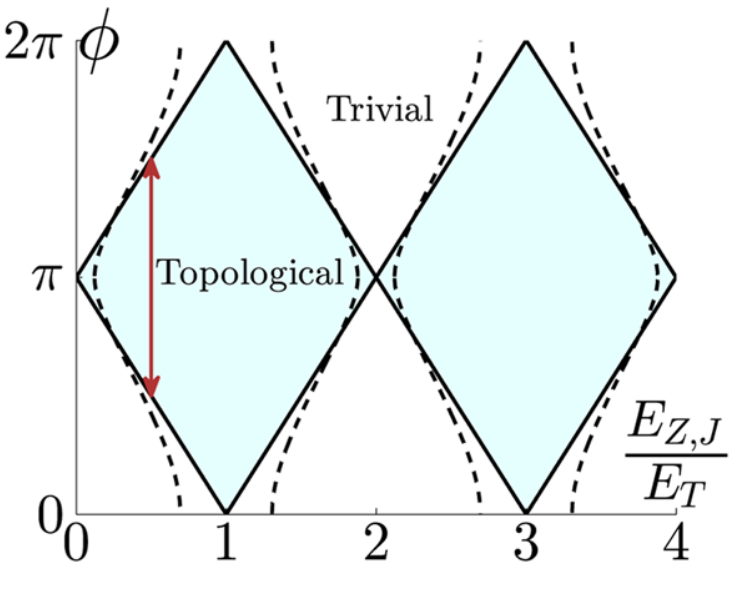
\includegraphics[width=0.5\columnwidth]{figures/pientka_phase_diagram}
		\caption{Phase vs. Magnetic field. Source\cite{pientka_topological_2017}}
		\label{fig:pientka_phase_diagram}
		\end{figure}
			
	\subsection{Bandstructure of a typical system}
		In Figure \ref{fig:pientka_bandstructure}, the bandstructure is displayed for the SNS system.
		Note that the gap is lowest at the Rashba/Zeeman split fermi-surface, where the momentum in the x direction equals $k_{F,1}$ or $k_{F,2}$.
		It is at these momenta that the wavefunctions are completely parallel to the translationally invariant direction, causing weak couipling with the superconductors.

		\begin{figure}[!htb]
		\centering
		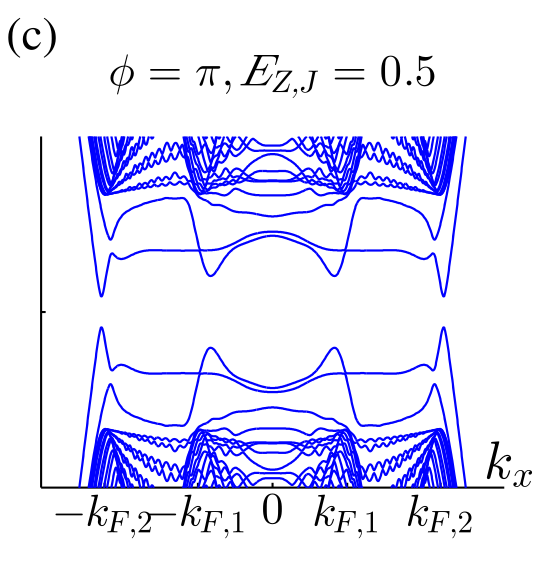
\includegraphics[width=0.5\columnwidth]{figures/pientka_bandstructure}
		\caption{Bandstructure of a straight SNS system~\cite{pientka_topological_2017}.
		Note that the gap is smallest at $k_{F,1}$ and $k_{F,2}$, which correspond to the two different Fermi momenta.}
		\label{fig:pientka_bandstructure}
		\end{figure}